\cleardoublepage

\begin{frontmatter}
	\chapter{Método das Forças (ou da Flexibilidade)}
\end{frontmatter}

\section{Equações de Equilíbrio}

Neste caso, as equações que descrevem um sistema estrutural são escritas em termos de ações desconhecidas (reações ou esforços internos). Para estruturas estaticamente determinadas (isostáticas), o sistema de equações nada mais é do que um conjunto de equações de equilíbrio derivadas das seguintes equações gerais:

\begin{minipage}{0.45\textwidth}
	\begin{equation} \label{syst1}
		\left\{
		\;
		\begin{aligned}
			\Sigma F_x & =0 \\
			\Sigma F_y & =0 \\
			\Sigma F_z & =0 \\
			\Sigma M_x & =0 \\
			\Sigma M_y & =0 \\
			\Sigma M_z & =0\end{aligned}
		\right.
	\end{equation}
\end{minipage}
\begin{minipage}{0.5\textwidth}
	\centering
	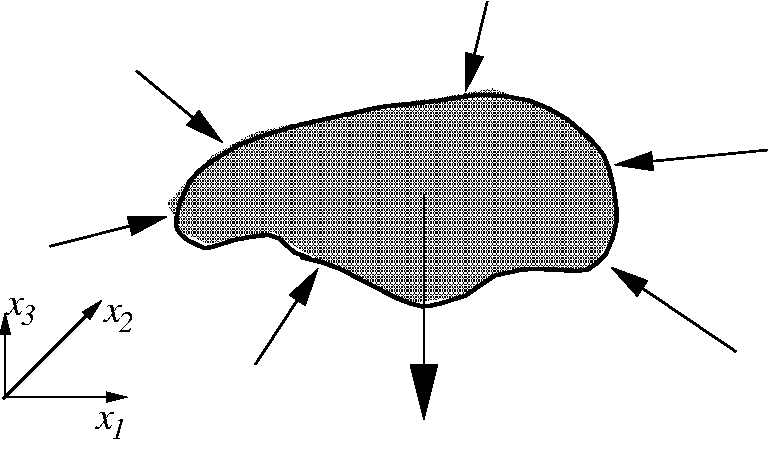
\includegraphics[scale=0.40]{img/solid3D}
	\captionof{figure}{Sólido geral.}
\end{minipage}

\bigskip

Por exemplo, para subsestruturas de pórticos planos (localizados no plano \(xy\)), tem-se as equações:

\bigskip

\begin{minipage}{0.45\textwidth}
	\[
		\left\{
		\;
		\begin{matrix}
			\Sigma F_x=0 \\
			\Sigma F_y=0 \\
			\Sigma M_z=0
		\end{matrix}
		\right.
	\]
\end{minipage}
\begin{minipage}{0.5\textwidth}
	\centering
	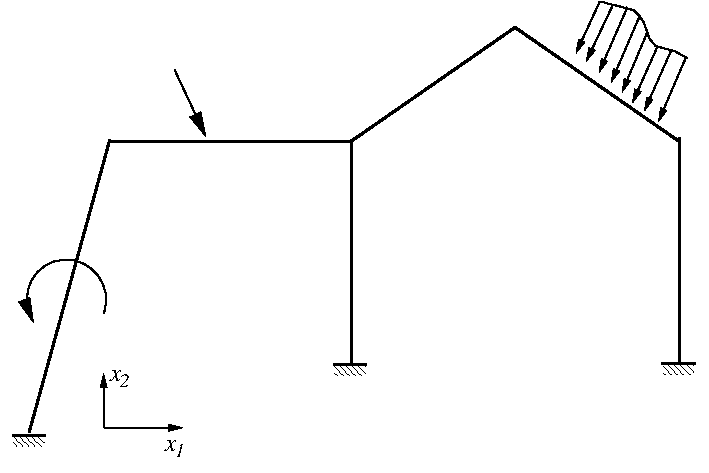
\includegraphics[scale=0.60]{img/porticoplano}
	\captionof{figure}{Pórtico plano.}
	\vspace{12pt}
\end{minipage}

\noindent Note que pelo tipo de problema, as equações \(\Sigma F_z=0\), \(\Sigma M_x=0\) e \(\Sigma M_y=0\) são meras identidades, pois pela definição do problema não há forças na direção de \(z\) e por conseguinte, também não há momentos segundo \(x\) ou \(y\). Essas equações não precisam, portanto, ser consideradas. No caso da existência de rótulas em seções do interior da estrutura (não nos apoios), equações adicionais de momento podem ser estabelecidas. Ressalta-se ainda que essas mesmas equações se aplicam na resolução de vigas.

Para outros tipos de estruturas reticuladas, indicam-se abaixo as equações de equilíbrio pertinentes

\bigskip

\begin{minipage}{0.25\textwidth}
	\underline{Treliças Planas}
	\bigskip
	\[
		\left\{
		\;
		\begin{matrix}
			\Sigma F_x=0 \\
			\Sigma F_y=0
		\end{matrix}
		\right.
	\]
\end{minipage}
\hspace{-1.5cm}
\begin{minipage}{0.7\textwidth}
	\centering
	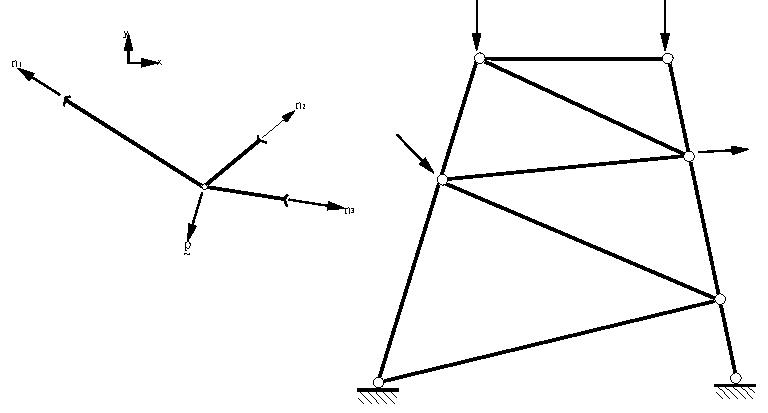
\includegraphics[scale=0.7]{img/trelicas2D}
	\captionof{figure}{Treliças planas.}
	\vspace{12pt}
\end{minipage}

Considerando-se um método baseado no equilíbrio nodal de forças, tem-se por nó que \(\Sigma F_x=0\) e \(\Sigma F_y=0\). Neste caso, também, \(\Sigma M_z=0\) é uma mera identidade, pois as ações em questão concorrem em um mesmo ponto (que é o próprio nó).

\bigskip

\begin{minipage}{0.25\textwidth}
	\underline{Grelhas}
	\bigskip
	\[
		\left\{ \;
		\begin{matrix}
			\Sigma M_x=0 \\
			\Sigma M_y=0 \\
			\Sigma F_z=0
		\end{matrix}
		\right.
	\]
\end{minipage}
\begin{minipage}{0.7\textwidth}
	\centering
	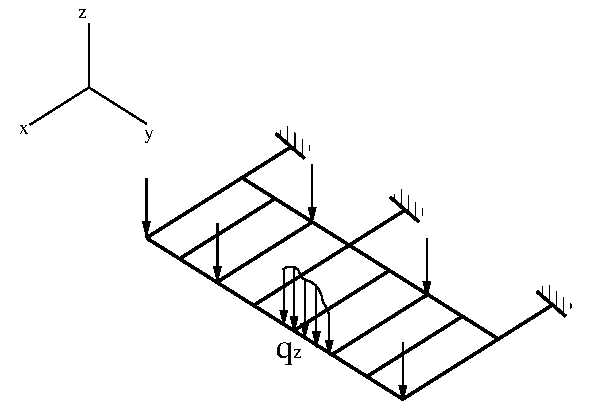
\includegraphics[scale=0.70]{img/grelha}
	\captionof{figure}{Grelhas.}
	\vspace{12pt}
\end{minipage}

\begin{minipage}{0.25\textwidth}
	\underline{Treliças espaciais}
	\bigskip
	\[
		\left\{ \;
		\begin{matrix}
			\Sigma F_x=0 \\
			\Sigma F_y=0 \\
			\Sigma F_z=0
		\end{matrix}
		\right.
	\]
\end{minipage}
\begin{minipage}{0.7\textwidth}
	\centering
	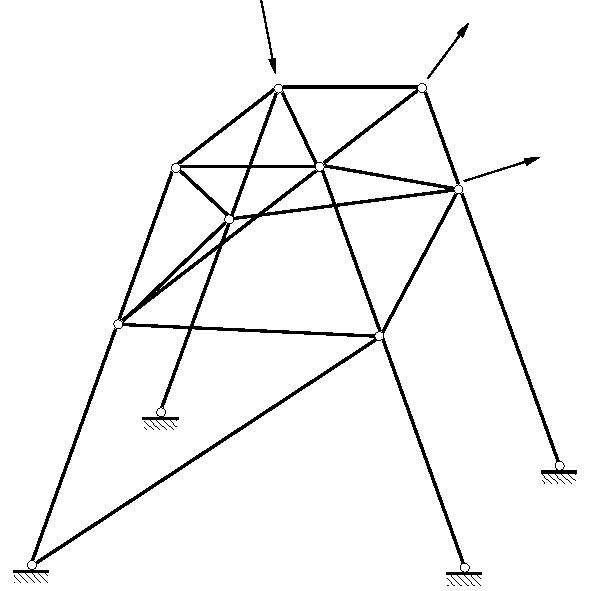
\includegraphics[scale=0.60]{img/trelica3D}
	\captionof{figure}{Treliças espaciais.}
	\vspace{12pt}
\end{minipage}

\clearpage

\begin{minipage}{0.25\textwidth}
	\underline{Pórticos espaciais}
	\bigskip
	\[
		\left\{ \;
		\begin{matrix}
			\Sigma F_x=0 \\
			\Sigma F_y=0 \\
			\Sigma F_z=0 \\
			\Sigma M_x=0 \\
			\Sigma M_y=0 \\
			\Sigma M_z=0
		\end{matrix}
		\right.
	\]
\end{minipage}
\begin{minipage}{0.7\textwidth}
	\centering
	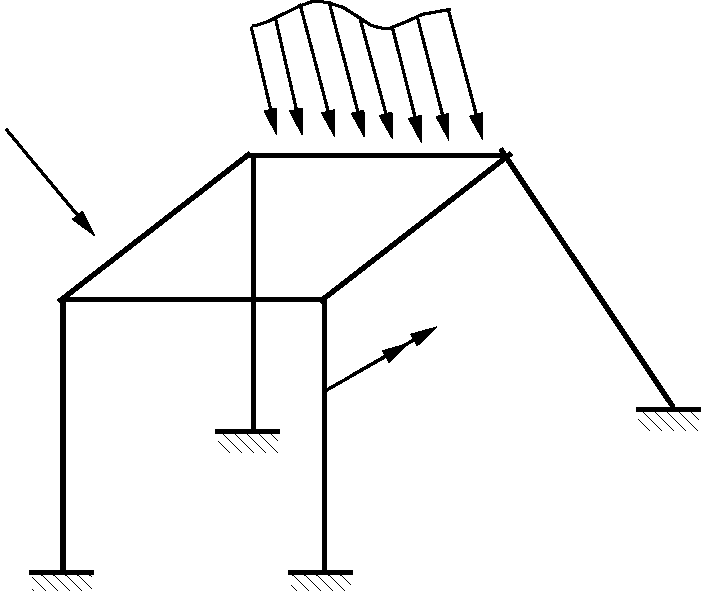
\includegraphics[scale=0.60]{img/portico3D}
	\captionof{figure}{Pórticos espaciais.}
	\vspace{12pt}
\end{minipage}

Para sistemas estruturais estaticamente indeterminados (hiperestáticos), há redundantes estáticas (ações que excedem o número de equações de equilíbrio pertinentes). Assim, além das equações de equilíbrio, anteriormente mostradas para os demais tipos de estruturas reticuladas, precisam ser consideradas equações adicionais de compatibilidade (de deslocamento), que são então usadas na determinação das redundantes estáticas.

\section{Equações de compatibilidade (de deslocamentos)}

Estas equações são assim denominadas porque exprimem ou impõem à solução condições relacionadas aos deslocamentos da estrutura. Para a sua obtenção, procede-se como se indica genericamente abaixo:

\begin{enumerate}
	\item
	      Rompe-se o sistema estrutural convenientemente de modo que sejam expostas todas as redundantes estáticas (ações incógnitas). Define-se, assim, o sistema principal.
	\item
	      Calculam-se, então, os deslocamentos na direção das correspondentes redundates estáticas (hiperestáticos) em função do agente externo solicitante (carregamento, variação de temperatura, recalque diferencial ou deformação inicial do elemento) e dos hiperestáticos.
	\item
	      Estabelecem-se então as equações de compatibilidade impondo-se a condição de deslocamento que há na direção de cada hiperestático. Haverá tantas equações quantos forem os hiperestáticos do problema.
	\item
	      Com os hiperestáticos calculados, tem-se então um problema isostático, que poderá ser resolvido via aplicação direta de equações de equilíbrio.
\end{enumerate}

Esquematicamente, o Método das Forças apresenta o fluxograma geral mostrado na Fig. \ref{fluxo-MF}.

\clearpage
\begin{figure}[!htbp]
	\centering
	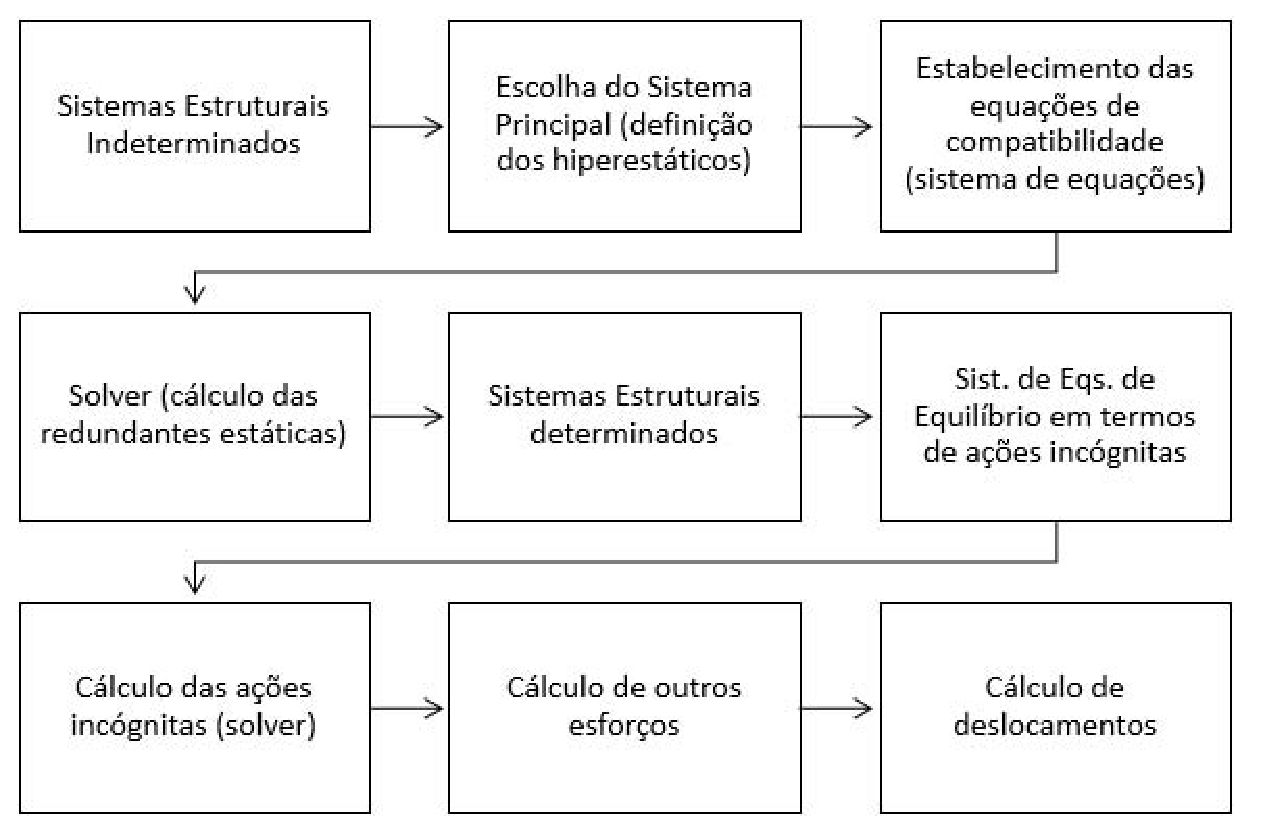
\includegraphics[scale=0.6]{img/fluxogramaMF}
	\caption{Fluxograma de análise segundo o Método das Forças.}
	\label{fluxo-MF}
\end{figure}

\section{O Sistema de equações (de compatibilidade)}

Havendo \(n\) redundantes estáticas (hiperestáticos), faz-se necessário romper a estrutura em \(n\) seções, quando da definição do sistema principal. Arbitrando-se, inicialmente, hiperestáticos unitários, ou seja, fazendo-se \(x_i=1\), \(i=1, 2, ..., n\), pode-se, então, via princípio dos trabalhos virtuais, calcular os deslocamentos \(\delta_{i0}\) e \(\delta_{ij}\), \(i,j=1, 2, ..., n\), quais denotam, respectivamente, os deslocamentos na direção \(x_i\) causados pelo agente externo (cargas, por exemplo) e pelo hiperestático \(x_j=1\). Resulta assim, para problemas lineares, o seguinte sistema de equações algébricas:

\par\bigskip
\(\delta_{i0}+\sum_{j=1}^{n}\delta_{ij}x_j=\delta_{i}\), com \(i=1, 2, ..., n \; ,\)
\par\bigskip

\noindent em que \(\delta_{i}\) é o deslocamento real na direção de \(x_i\). Os coeficientes \(\delta_{ij}\) são denominados de coeficientes de flexibilidade ou simplesmente de flexibilidades. Em notação matricial, o sistema de equações de compatibilidade pode ser escrito como:

\par\bigskip

\begin{minipage}{0.6\textwidth}
\(
\left[ \;\;
	\begin{matrix}
		\delta_{11} & \delta_{12} & \cdots      & \delta_{1n} \\
		\delta_{21} & \delta_{22} & \cdots      & \delta_{2n} \\
		\vdots      & \vdots      & \ddots      & \vdots      \\
		\delta_{n1} & \delta_{n2} & \delta_{11} & \delta_{nn}
	\end{matrix}
	\right]
\)
\(
\begin {Bmatrix}
\; x_1 \\
\; x_2 \\
\vdots  \\
\;\;  x_n  \end{Bmatrix}=\begin{Bmatrix}
	\delta_1 \\
	\delta_2 \\
	\vdots   \\
	\;\; \delta_n\end{Bmatrix}-\begin{Bmatrix}
	\;\delta_{10} \\
	\;\delta_{20} \\
	\vdots        \\
	\;\delta_{n0}
\end{Bmatrix} \; ; \quad
\)
\end{minipage}
\begin{minipage}{0.35\textwidth}
	\(\mathbf{F} \cdot \mathbf{x} \;=\; \boldsymbol{\delta}-\boldsymbol{\delta}_0
	\; ,\)
\end{minipage}

\par\bigskip

\noindent onde \(\mathbf{F}\) é a chamada matriz de flexibilidade do sistema estrutural. Exprimindo-se, conjuntamente, equações de compatibilidade e de equilíbrio, sendo estas últimas necessárias à determinação das outras incógnitas do problema (reações e esforços internos não redundantes), tem-se:

\par\bigskip
\(
\left [\;\, \begin{matrix}
		\mathbf{F}      & \mathbf{0}      \\
		\mathbf{A}_{r1} & \mathbf{A}_{rr}
	\end{matrix}
	\right ]\begin{Bmatrix}
	\; \mathbf{x}
	\\
	\mathbf{r}
\end{Bmatrix}=\begin{Bmatrix}
	\;\, \boldsymbol{\delta}-\boldsymbol{\delta}_0
	\\
	\mathbf{b}
\end{Bmatrix}  \; ,
\)
\par\bigskip

\noindent em que \(\textbf{b}\) é um vetor associado ao carregamento atuante na estrutura e \(\mathbf{A}_{r1}\) e \(\mathbf{A}_{rr}\) são submatrizes que resultam do estabelecimento das equações de equilíbrio do sistema estrutural principal.

\newpage

Observações:
\begin{enumerate}
	\item
	      Do teorema de reciprocidade de Betti-Rayleigh, sabe-se que \(\delta_{ij}=\delta_{ji}\). Para estruturas reticuladas este teorema pode ser facilmente demonstrado via P.F.V. (princípio das forças virtuais). Tem-se, em geral:

	      \bigskip

	      \[
		      \begin{aligned}
			      \delta_{ij}
			       & =
			      \int_{L}\frac{\bar{M}_iM_j}{k_b}ds
			      +\int_{L}\frac{\bar{N}_iN_j}{k_a}ds
			      +\int_{L} \frac{\bar{Q}_iQ_j}{k_s}ds
			      +\int_{L}\frac{\bar{M}_{ti}M_{tj}}{k_t}ds \\ & =
			      \int_{L}\frac{M_i\bar{M}_j}{k_b}ds
			      +\int_{L}\frac{N_i\bar{N}_j}{k_s}ds
			      +\int_{L}\frac{Q_i\bar{Q}_j}{k_s}ds
			      +\int_{L}f
			      \frac{M_{ti}\bar{M}_{tj}}{k_t}ds
			      =
			      \delta_{ji}
		      \end{aligned} \; ,
	      \]

	      \bigskip

	      \noindent uma vez que sendo \(x_i=x_j=1\), então \(\bar{M}_i=M_i\), \(\bar{M}_j=M_j\), \(\bar{N}_i=N_i\), \(\bar{N}_j=N_j\) e assim por diante. Na equação acima, \(k_b=EI_z\), \(k_a=EA\), \(k_s=GA_s\) e \(k_t=GJ_t\) denotam, respectivamente, as rigidezes flexional, axial, transversal e torcional em seções do elemento (aqui consideradas particularmente de materiais homogêneos).\

	\item
	      Note-se que as variáveis \(\bf{x}\) e \(\bf{r}\) são desacopladas. Para a sua resolução, primeiro calcula-se \(\bf{x}\), e de posse de \(\bf{x}\), calcula-se \(\bf{r}\). Tem-se:

	      \bigskip

	      \(\left\{\begin{aligned}
		      \mathbf{x} & =\mathbf{F}^{-1}(\boldsymbol{\delta}-\boldsymbol{\delta}_0) \\
		      \mathbf{r} & =\mathbf{A}_{rr}^{-1}(\mathbf{b}-\mathbf{A}_{r1}\bf{x})
	      \end{aligned}\right.\)

	      \bigskip

	\item
	      Eventuais hipostaticidades no sistema estrutural serão detectadas analisando-se o determinante de \(\bf{A}_g\), que denota a matriz global do sistema estrutural. Vale:
	      Se \(\left |\bf{A}_g  \right |=0\), então o sistema estrutural será hipostático.
\end{enumerate}

\section{Efeitos de variação de temperatura, deformação inicial, protensão e recalque de apoio}

\subsection{Variação de temperatura}

Havendo \(n\) redundantes na estrutura, incluem-se efeitos de variação de temperatura pela determinação do vetor \(\delta_{it}\), que expressa o deslocamento na direção da redundante \(x_i\), no sistema principal, em consequência de uma certa variação de temperatura.
Ressalta-se que as variações de temperatura ou geram deformações axiais nos elementos (caso de variação uniforme de temperatura) ou geram deformações flexionais (caso de variação diferencial de temperatura).

Em geral, tem-se para a consideração de efeitos de temperatura as expressões mostradas juntamente com a Fig. \ref{def-temp}, compatíveis com aumentos de temperatura (\(t_i, t_s, t_g\) positivos).
\begin{figure}[!ht]
	\begin{center}
		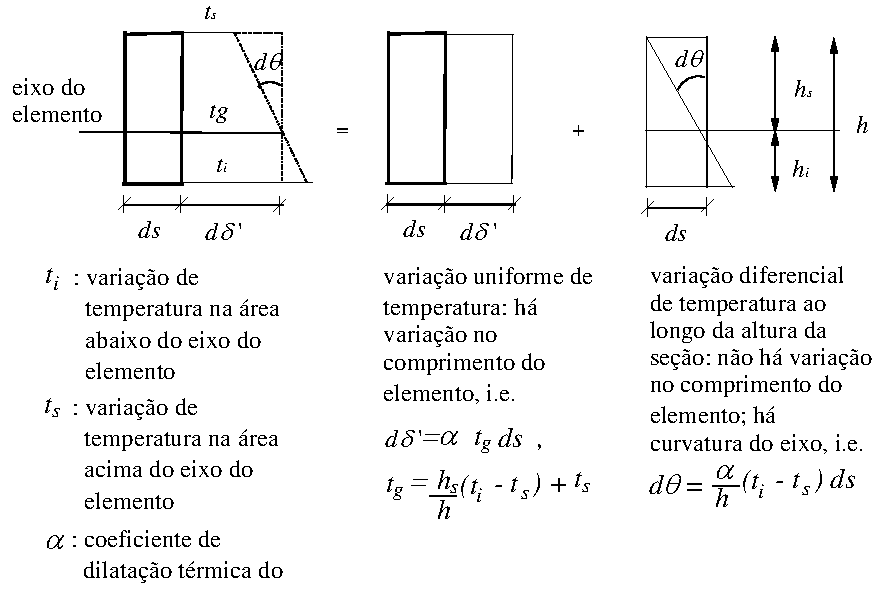
\includegraphics[scale=0.7]{img/temperatura}
		\caption{Deformações em razão da temperatura.}
		\label{def-temp}
	\end{center}
\end{figure}

\subsection{Deformação Inicial}

Incluem-se efeitos de deformações iniciais por processo idêntico ao adotado para a consideração de variações de temperatura. Afinal de contas, um elemento com comprimento diferente do de projeto gerará, na estrutura, efeitos idênticos àqueles provocados por uma variação uniforme de temperatura que produzisse tal comprimento real do elemento. Do mesmo modo, uma curvatura inicial em um elemento corresponde, identicamente, a uma variação diferencial de temperatura entre bordas superior e inferior de seções da estrutura. Assim, para a inclusão de tais efeitos na análise, calcula-se o vetor \(\delta_{id}\), que exprime o deslocamento, no sistema principal, na direção da redundante \(x_i\) em função de deformações iniciais (\(\delta_0\) ou  \(\theta_0\)).

Note-se que no caso de variação de temperatura faz-se necessário determinar, pelas expressões pertinentes, o campo de deslocamentos associado; no caso de deformações iniciais esses campos são diretamente fornecidos.

Sob deformações inciais, obviamente também se incluem as deformações e correspondentes tensões originadas em razão da deformação lenta (creep) ou retração (shrinkage) no concreto, que solicitam a estrutura devido a restrições das deformações envolvidas --- que ocorreriam se pudessem se deformar livremente. Este é também o caso da relaxação de protensão (perda de tração no aço protendido) em elementos manufaturados em concreto protendido.

\subsection{Recalques de Apoio (condições de contorno não-homogêneas)}

Neste caso há duas situações. Se o deslocamento prescrito corresponder à direção de uma redundante, então poderá ser diretamente considerado no vetor de deslocamentos reais da estrutura, \(\mathbf{\delta}\) (vide sistema de equações de compatibilidade). Por outro lado, caso o deslocamento de apoio não corresponda a nenhuma das redundantes selecionadas, então poderá ser incorporado à análise via cálculo do vetor \(\delta_{ir}\), que conterá, a exemplo dos casos anteriores, o deslocamento na direção da redundante \(x_i\) em decorrência dos valores prescritos de deslocamento (recalques).

\subsection{Sistema de Equações de Compatibilidade}

Para problemas lineares (situação em que vale o princípio da superposição de efeitos), o sistema de equações de compatibilidade, nas situações mais gerais, é da forma:

\[
	\mathbf{F} \cdot \mathbf{x}
	=
	\boldsymbol{\delta}
	-\boldsymbol{\delta}_0
	-\boldsymbol{\delta}_t
	-\boldsymbol{\delta}_d
	-\boldsymbol{\delta}_r
\]

\section{Sistemas Estruturais com Elementos de Rigidez Variável}

Neste caso, as integrais de linhas que surgem na expressão matemática do princípio dos trabalhos virtuais (usado para cálculo de deslocamentos e por conseguinte, para a determinação dos coeficientes da matriz de flexibilidade e do termo independente) poderão, raramente, ser calculadas analiticamente. Exemplos de tais integrais são:

\[
	\int_{L}\frac{M_i\overline{M}_j}{k_b}ds \;,\quad
	\int_{L}\frac{N_i\overline{N}_j}{k_a}ds \;,\quad
	\int_{L}\frac{Q_i\overline{Q}_j}{k_s}ds \;,\quad
	\int_{L}\frac{M_{ti}\overline{M}_{tj}}{k_t}ds  \; ,
\]

\noindent onde  \(k_b\), \(k_a\), \(k_s\) e \(k_t\) denotam, respectivamente, as rigidezes flexional, axial, transversal (ao cisalhamento) e torcional em seções do elemento. Para casos particulares de variação de rigidez (por exemplo, mísulas cuja altura varia linearmente ou parabolicamente) e cargas (concentradas ou uniformemente distribuídas, por exemplo), há tabelas que fornecem os resultados de algumas das integrais acima, que eram comumente usadas em cálculos manuais. Todavia, atualmente, na era computacional, tais tablas são desnecessárias e as  integrais envolvidas podem ser confortável e precisamente avaliadas via estratégias numéricas de integração. Por exemplo, via quadratura de Gauss-Legendre. Tem-se:

\[
	\int_{L}\frac{M_i\overline{M}_j}{k_b}ds
	=
	int_{-1}^{+1}f[x(r)]\cdot|J(r)|dr
	=
	\sum_{k=1}^{npg}f(r_k)\cdot|J(r_k)|\cdot w_k
\]

\noindent onde,

\[
	f[x(r)]
	=
	\frac{M_i(x)\overline{M}_j(x)}{k_b(x)}, \qquad
	|J(r)|=\frac{ds}{dr}
\]

\noindent sendo \(r_k\) a abcissa do \(k\)-ésimo ponto de integração, e \(w_k\), o respectivo peso. Usualmente, não mais que três pontos de integração (\(npg=3\)) são necessários para uma avaliação precisa das integrais. Note ainda que para elementos lineares (com 2 nós), \(|J(r)|=\frac{l_e}{2}\)

\section{Fator de forma ao cisalhamento (\(\chi\))}

Seja o elemento estrutural abaixo, em que se analisa a deformação por cisalhamento na direção \(y\), um dos eixos principais da seção (vide Fig. \ref{shear-ef}).

\begin{figure}[!htbp]
	\centering
	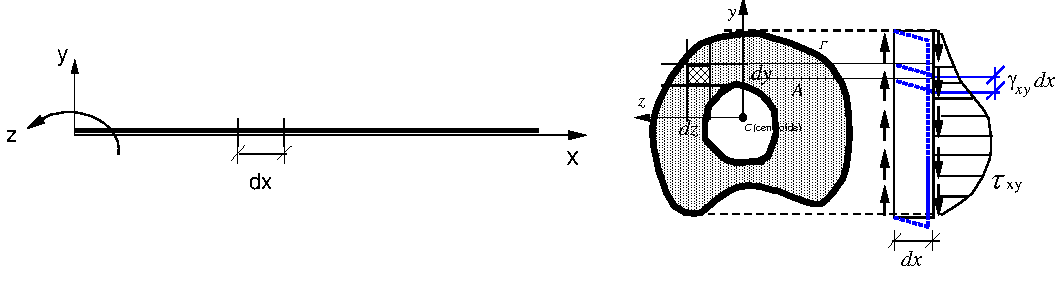
\includegraphics[scale=0.70]{img/shearfactor}
	\caption{Consideração de efeitos de cisalhamento.}
	\label{shear-ef}
\end{figure}

\noindent A parcela de trabalho virtual interno associado à tensão \(\tau_{xy}\), em um infinitesimal de elemento \(dx\), é dado por:

\[
	dW_{int}(\tau_{xy})
	=
	(\overline{\tau}_{xy}\cdot dy\cdot dz)
	(\gamma_{xy}\cdot dx)
	=
	(G\cdot \overline{\gamma}_{xy}\cdot dy\cdot dz)
	(\gamma_{xy}\cdot dx)
	\; ,
\]

\noindent com

\begin{minipage}{0.5\textwidth}
	\[
		\hspace{2.0cm}
		\begin{aligned}
			 & \gamma_{xy}(y)=\frac{\tau_{xy}(y)}{G}=\frac{Q_yM_{sz}(y)}{GI_zb(y)} \;, \\
			 & M_{sz}(y)=\int_{y}^{y_t}s \cdot b(s) \cdot ds \;,
		\end{aligned}
	\]
\end{minipage}
\begin{minipage}{0.4\textwidth}
	\begin{center} \hspace{-1.0cm}
		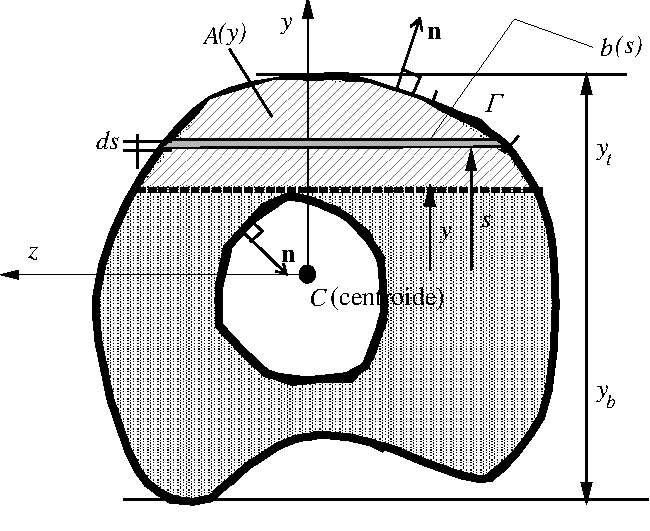
\includegraphics[scale=0.40]{img/statmom}
		\captionof{figure}{Momento estático, \(M_{st}(y)\).}
		\label{mom_st}   \vspace{12pt}
	\end{center}
\end{minipage}

\noindent sendo \(M_{sz}(y)\) o momento estático de \(A(y)\) em relação à linha neutra \(z\),  \(d\overline{Q}_y=\overline{\tau}_{xy}\cdot dy\cdot dz\) o infinitesimal de cortante devido à carga unitária, \(\overline{P}=1\),  \(d\overline{\lambda}_y=\overline{\gamma}_{xy}\cdot dx\) o deslizamento relativo associado \(\bar{Q}_{y}\), e \(d\lambda_y=\gamma_{xy}\cdot dx\) o deslizamento  relativo  real.

\medskip

\noindent Assim, para uma dada seção \(x\) do elemento, tem-se:

\medskip

\[ \begin{aligned}
		\frac{dW_{int}(x)}{dx}
		 & =G \cdot \int_{A(x)} \frac{\overline{Q}_y \cdot M_{sz}(y)}{G\cdot I_{z}b(y)}\cdot \frac{Q_{y} \cdot M_{sz}(y)}{G\cdot I_{z}b(y)}dz\cdot dy                                                                              \\
		 & =\int_{-y_b}^{y_t}\int_{0}^{b(y)} \frac{\overline{Q}_y \cdot Q_y \cdot M_{sz}^2(y)}{G\cdot I_{z}^2\cdot b^2(y)}dz\cdot dy                                                                                               \\
		 & =\int_{-y_b}^{y_t} \frac{\overline{Q}_y \cdot Q_y \cdot M_{sz}^2(y)}{G\cdot I_{z}^2\cdot b(y)}dy =\frac{\overline{Q}_y \cdot Q_y}{G \cdot A}\left[ \frac{A}{I_z^2} \int_{-y_b}^{y_t}\frac{M_{sz}^2(y)}{b(y)} dy \right] \\
		 & =\frac{\overline{Q}_y \cdot Q_y}{G \cdot A}\cdot \chi_y  =\frac{\overline{Q}_y \cdot Q_y}{G \cdot A_{sy}}
	\end{aligned}
\]

\medskip

\noindent sendo \(A_{sy}=({A}/{\chi_y})\) a área de cisalhamento efetiva na direção \(y\) e \(\chi_y\) o fator de forma ao cisalhamento na direção \(y\), dado por

\[
	\chi_y
	=
	\frac{A}{I_z^2} \int_{-y_b}^{y_t}\frac{M_{sz}^2(y)}{b(y)} dy=\frac{A}{A_{sy}}
	\; ; \quad
	A_{sy}
	=
	\frac{I_z^2}{\int_{-y_b}^{y_t}\frac{M_{sz}^2(y)}{b(y)} dy}
	\; .
\]

